\documentclass{article}
\usepackage{tikz}
\usetikzlibrary{positioning}

\begin{document}

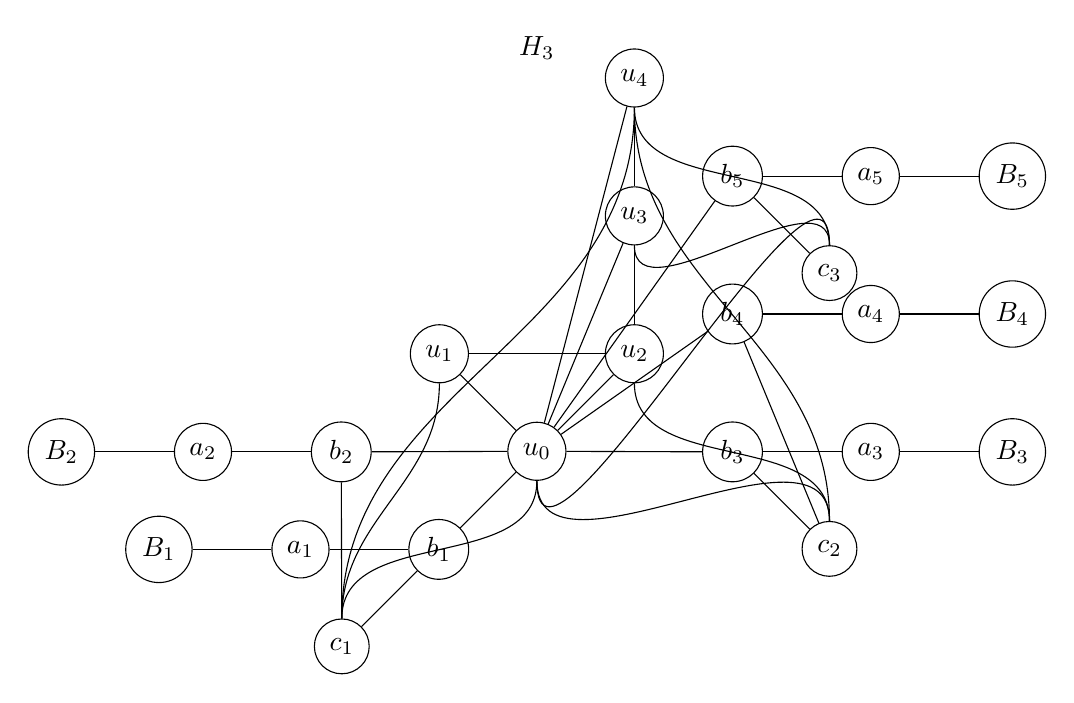
\begin{tikzpicture}[node distance=1cm, auto]
    % Define nodes
    \node (u0) [circle, draw] {$u_0$};
    \node (u1) [circle, draw, above left=of u0] {$u_1$};
    \node (u2) [circle, draw, above right=of u0] {$u_2$};
    \node (u3) [circle, draw, above=of u2] {$u_3$};
    \node (u4) [circle, draw, above=of u3] {$u_4$};
    
    \node (b1) [circle, draw, below left=of u0] {$b_1$};
    \node (b2) [circle, draw, below left=of u1] {$b_2$};
    \node (b3) [circle, draw, below right=of u2] {$b_3$};
    \node (b4) [circle, draw, below right=of u3] {$b_4$};
    \node (b5) [circle, draw, below right=of u4] {$b_5$};
    
    \node (c1) [circle, draw, below left=of b1] {$c_1$};
    \node (c2) [circle, draw, below right=of b3] {$c_2$};
    \node (c3) [circle, draw, below right=of b5] {$c_3$};
    
    \node (a1) [circle, draw, left=of b1] {$a_1$};
    \node (a2) [circle, draw, left=of b2] {$a_2$};
    \node (a3) [circle, draw, right=of b3] {$a_3$};
    \node (a4) [circle, draw, right=of b4] {$a_4$};
    \node (a5) [circle, draw, right=of b5] {$a_5$};
    
    \node (B1) [circle, draw, left=of a1] {$B_1$};
    \node (B2) [circle, draw, left=of a2] {$B_2$};
    \node (B3) [circle, draw, right=of a3] {$B_3$};
    \node (B4) [circle, draw, right=of a4] {$B_4$};
    \node (B5) [circle, draw, right=of a5] {$B_5$};
    
    % Draw edges
    \draw (u0) -- (u1);
    \draw (u0) -- (u2);
    \draw (u0) -- (u3);
    \draw (u0) -- (u4);
    
    \draw (u1) -- (u2);
    \draw (u2) -- (u3);
    \draw (u3) -- (u4);
    
    \draw (u0) -- (b1);
    \draw (u0) -- (b2);
    \draw (u0) -- (b3);
    \draw (u0) -- (b4);
    \draw (u0) -- (b5);
    
    \draw (b1) -- (c1);
    \draw (b2) -- (c1);
    \draw (b3) -- (c2);
    \draw (b4) -- (c2);
    \draw (b5) -- (c3);
    
    \draw (a1) -- (b1);
    \draw (a2) -- (b2);
    \draw (a3) -- (b3);
    \draw (a4) -- (b4);
    \draw (a5) -- (b5);
    
    \draw (B1) -- (a1);
    \draw (B2) -- (a2);
    \draw (B3) -- (a3);
    \draw (B4) -- (a4);
    \draw (B5) -- (a5);
    
    \draw (u0) to[out=-90,in=90] (c1);
    \draw (u0) to[out=-90,in=90] (c2);
    \draw (u0) to[out=-90,in=90] (c3);
    
    \draw (u1) to[out=-90,in=90] (c1);
    \draw (u2) to[out=-90,in=90] (c2);
    \draw (u3) to[out=-90,in=90] (c3);
    
    \draw (u4) to[out=-90,in=90] (c1);
    \draw (u4) to[out=-90,in=90] (c2);
    \draw (u4) to[out=-90,in=90] (c3);
    
    \node at (current bounding box.north) {$H_3$};
\end{tikzpicture}

\end{document}